%------------------------------------------------
\section{Ant colony system}
%------------------------------------------------

\begin{frame} \frametitle{Ant colony} 

\begin{itemize}[<+->]
	\item Meta-heuristic proposed by [Colorni, et Al], improved by [Dorigo, Gambardella, et al.]
	\item Mimicry of ants behavior to find optimal path between nest and food
	\begin{itemize}
		\item Transition rules
	\end{itemize}
	\item Indirect communication between ants through pheromones amount
	\begin{itemize}
		\item Update rules
	\end{itemize}
	\item State of the art in various optimization problem
\end{itemize}

\end{frame}


\begin{frame}\frametitle{Ant exaple}
\begin{figure}[t]
	\label{fig:ants}
	\centering
	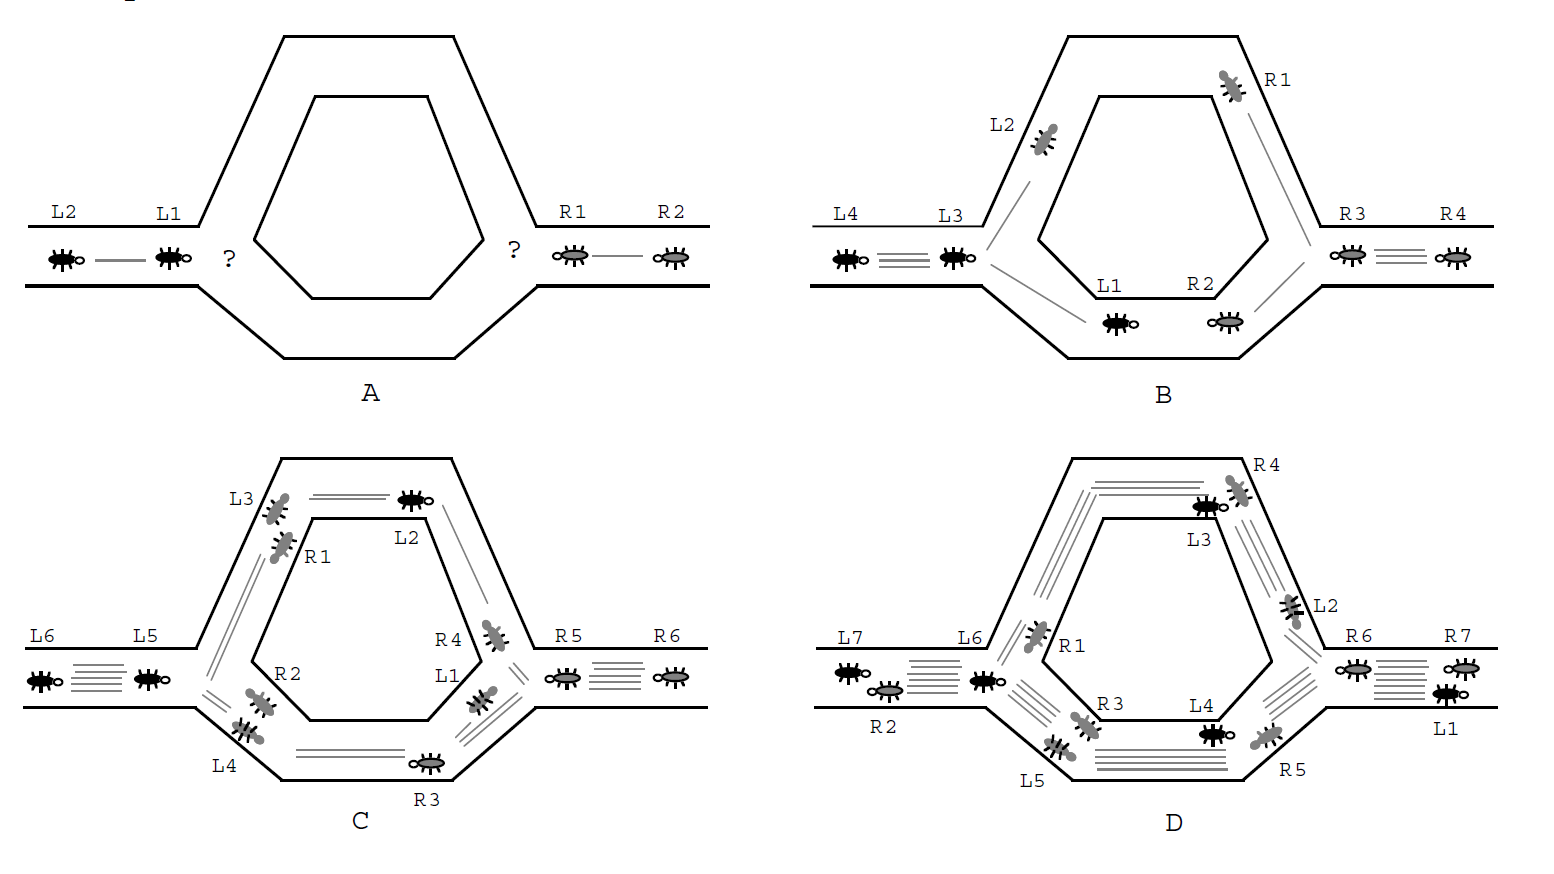
\includegraphics[width=.75\columnwidth]{ants_example}
	\caption{How real ants find a shortest path [Dorigo, Gambardella, et al.].}
\end{figure}
\end{frame}


\begin{frame} \frametitle{Transition rules} 

\begin{block}{Ant Colony Optimization}
\begin{equation*}
P_{ij}^{k} = \frac{\tau_{ij}^{\alpha}~\eta_{ij}^{\beta}}{\sum_{l\in\Psi}\tau_{il}^{\alpha}~\eta_{il}^{\beta}}
\end{equation*}	
\end{block}

\begin{block}{Ant Colony System}
Pseudo random proportional rule:
\begin{equation*}
j = 
\begin{cases} 
\displaystyle\operatorname*{arg\,max}_{j\in J(i)} \{ {[\tau_{ij}]\cdot[\eta_{ij}]^{\beta}} \} & \text{if } q\leq q_0 \quad\quad \text{(exploitation)} \\
S & otherwise \quad \text{(biased exploration)}
\end{cases}
\end{equation*}
where $S$ is a random variable selected according to $P_{ij}^{k}$ 
\end{block}

\end{frame}



\begin{frame} \frametitle{Update rules} 

\begin{block}{Global update rule}
\begin{equation*}
\tau_{ij} \leftarrow (1 - \alpha)\cdot\tau_{ij}~+~\alpha\cdot\tau_{ij}^{k}
\end{equation*}

\begin{equation*}
\Delta\tau_{ij}^{k} = 
\begin{cases} 
1/L_{gb} & \text{if arc}~(i,j)\in~\text{global-best-tour} \\
0		 & \text{Otherwise}
\end{cases}
\end{equation*}

\end{block}

\begin{block}{Local update rule}

\begin{equation*}
\tau_{ij} \leftarrow (1 - \rho)\cdot\tau_{ij}~+~\rho\cdot\tau_{ij}^{k}
\end{equation*}

\begin{equation*}
\Delta\tau_{ij}^{k} = 
\begin{cases} 
1/L_{init} 	& \text{if arc}~(i,j)\in~\text{initial-tour} \\
0    		& \text{Otherwise}
\end{cases}
\end{equation*}
\end{block}

\end{frame}


\begin{frame} \frametitle{Solution encoding} 

\begin{block}{Machine assignment}
\begin{equation} \label{eq:stage1} \tag{stage 1}
S_1 =[~3~2~3~1~4~3~4~2~1~4]
\end{equation}
(interpretation) machine three ($m_3$) has assigned jobs 1, 3 and 6
\end{block}

\begin{block}{Jobs sequencing}
\begin{equation}\label{eq:stage2} \tag{stage 2}
S_2 =
\begin{bmatrix}
9  &  4  &  0 &  0 &  0 &  0 &  0 &  0 &  0 &  0 \\
8  &  2  &  0 &  0 &  0 &  0 &  0 &  0 &  0 &  0 \\
6  &  3  &  1 &  0 &  0 &  0 &  0 &  0 &  0 &  0 \\
5  & 10  &  7 &  0 &  0 &  0 &  0 &  0 &  0 &  0 
\end{bmatrix}
\end{equation}	
(interpretation) machine one ($m_1$) will process jobs in the following order: $9 \rightarrow 4$
\end{block}

\end{frame}


\begin{frame} \frametitle{Transition definition (Stage 1)} 

\begin{block} {Transition rule}
\begin{equation}\label{eq:acsTauStage1} 
j = 
\begin{cases} 
\displaystyle\operatorname*{arg\,max}_{j\in J(i)} \{ {[\tau_{jk}^{I}]\cdot[\eta_{jk}^{I}]^{\beta}} \} & \text{if } q\leq q_0 \quad\quad \text{(exploitation)} \\
S & otherwise \quad \text{(biased exploration)}
\end{cases}
\end{equation}
\end{block}

\begin{block}{Visibility metric}
\begin{columns}[c]
	\begin{column}[c]{6cm}
	\begin{equation} \label{eq:acsEta1Stage1}
	\eta_{jk}^{I} = \frac{1}{P_{jk}}
	\end{equation}	
	\end{column}
	\pause
	\begin{column}[c]{6cm}
	\begin{equation} \label{eq:acsEta2Stage1}
	\eta_{jk}^{I} = \frac{1}{
		\left[ \frac{P_{jk}}{\operatorname*{max}_{m\in M_{j}}(P_{jm})} +
		\frac{E_{jk}}{\operatorname*{max}_{m\in M_{j}}(E_{jm})}\right]}
	\end{equation}
	[Tonelli, Salido, et al. 2016]
	\end{column}
\end{columns}
\end{block}

\end{frame}


\begin{frame} \frametitle{Transition definition (Stage 2)} 

\begin{block} {Transition rule}
\begin{equation} \label{eq:acsTauStage2}
j = 
\begin{cases} 
\displaystyle\operatorname*{arg\,max}_{j\in J(i)} \{ {[\tau_{ij}^{II,k}]\cdot[\eta_{ij}^{II,k}]^{\beta}} \} & \text{if } q\leq q_0 \quad\quad \text{(exploitation)} \\
S & otherwise \quad \text{(biased exploration)}
\end{cases}
\end{equation}
\end{block}

\begin{block}{Visibility metric}
	\begin{columns}[c]
		\begin{column}[c]{6cm}
		\begin{equation} \label{eq:acsEta1Stage2}
		\eta_{ij}^{II,k} = \frac{1}{s_{ijk}}
		\end{equation}
		\end{column}
		\pause
		\begin{column}[c]{6cm}
		\begin{equation} \label{eq:acsEta2Stage2}
		\eta_{ij}^{II,k} = \frac{1}{
			\left[ \frac{s_{ijk}}{\operatorname*{max}_{j'\in J_{k}}(s_{ij'k})} +
			\frac{r_{j}}{\operatorname*{max}_{j'\in J_{k}}(r_{j'})}\right]}
		\end{equation}
		\end{column}
	\end{columns}
\end{block}

\end{frame}


\begin{frame} \frametitle{Pheromone global update} 

\begin{block} {Stage 1}
\begin{equation} \label{eq:acsTauStage1UpdateGlobal}
\tau_{jk}^{I} \leftarrow (1 - \alpha)\cdot\tau_{jk}^{I} +\alpha\cdot\Delta\tau_{jk}^{I,Best}
\end{equation}

\begin{equation}
\Delta\tau_{jk}^{I,Best} = 
\begin{cases} 
1/F(s_{gb}) & \text{if arc}~(j,k)\in~\text{global-best-schedule} \\
0			& \text{Otherwise}
\end{cases}
\end{equation}

\end{block}

\begin{block}{Stage 2}

\begin{equation} \label{eq:acsTauStage2UpdateGlobal}
\tau_{ij}^{II,k} \leftarrow (1 - \alpha)\cdot\tau_{ij}^{II,k} +\alpha\cdot\Delta\tau_{ij}^{II,Best}
\end{equation}
\begin{equation}
\Delta\tau_{ij}^{II,Best} = 
\begin{cases} 
1/F(s_{gb}) & \text{if arc}~(i,j,k)\in~\text{global-best-schedule} \\
0			& \text{Otherwise}
\end{cases}
\end{equation}
\end{block}


\end{frame}


\begin{frame} \frametitle{Pheromone local update} 

\begin{block} {Stage 1}
\begin{equation} \label{eq:acsTauStage1UpdateLocal}
\tau_{jk}^{I} \leftarrow (1 - \rho)\cdot\tau_{jk}^{I} +\rho\cdot\Delta\tau_{jk}^{I,Best}
\end{equation}

	
\begin{equation}
\Delta\tau_{jk}^{I,Best} = 
\begin{cases} 
1/F(s_{init}) & \text{if arc}~(j,k)\in~\text{initial-best-schedule} \\
0			& \text{Otherwise}
\end{cases}
\end{equation}

	
\end{block}

\begin{block}{Stage 2}
	
\begin{equation} \label{eq:acsTauStage2UpdateLocal}
\tau_{ij}^{II,k} \leftarrow (1 - \rho)\cdot\tau_{ij}^{II,k} +\rho\cdot\Delta\tau_{ij}^{II,Best}
\end{equation}

\begin{equation}
\Delta\tau_{ij}^{II,Best} = 
\begin{cases} 
1/F(s_{init}) & \text{if arc}~(i,j,k)\in~\text{initial-best-schedule} \\
0			& \text{Otherwise}
\end{cases}
\end{equation}


\end{block}


\end{frame}


%\subsection{Local Search}

\begin{frame}[fragile] \frametitle{Local search procedure} 


\begin{algorithm}[H]
	\footnotesize
	\caption{Local search procedure}
	\label{alg:acoLocalSearch}
	Set $LocalIteration = 1$\;
	\While{$LocalIteration \leq MaxLocalterations$}{
		Generate random variable ($rv$) from $U(0,1)$\;
		\eIf{$rv < 0.5$}{
			generate neighboring solution for $S_1(Ant)$: $N_1(Ant) \wedge x = 1$\;
		}{
			generate neighboring solution for $S_2(Ant)$: $N_2(Ant) \wedge x = 2$
		}
		Determine $F(N_x(Ant))$\;
		\If{$F(N_x(Ant)) \leq F(Ant)$}{
			$S_x \leftarrow N_x(Ant)$\;
		}
		$LocalIteration = LocalIteration + 1$
	}
\end{algorithm}

\end{frame}


%\subsection{ACS workflow}

\begin{frame}[fragile] \frametitle{Ant colony system workflow} 

\begin{algorithm}[H]
	\footnotesize
	\caption{ACS workflow}
	\label{alg:acoWorkflow}
	Populate the paths with specified pheromone amounts $(\tau_{jk}^{I},\tau_{ij}^{II,k})$\;
	\While{$not~StopCriteria$}{
		Set $Step = 1$\;
		\While{$Step \leq MaxSteps$}{
			\For{$Ant \in Ants$}{
				Solve $Step$ for Stage 1 (Assignment): find $S_1$ according to \cref{eq:acsTauStage1,eq:acsEta1Stage1,eq:acsEta2Stage1}\;
				Solve $Step$ for Stage 2 (Sequencing): find $S_2$ according to \cref{eq:acsTauStage2,eq:acsEta1Stage2,eq:acsEta2Stage2}\;		
			}	
			Update pheromone amounts locally according to \cref{eq:acsTauStage1UpdateLocal,eq:acsTauStage2UpdateLocal}\; 
		}
		Calculate $F(Ants)$ that are associated with $S_1$ and $S_2$\;		
		Execute local search procedure for all ants\;
		Update pheromone amounts globally according to \cref{eq:acsTauStage1UpdateGlobal,eq:acsTauStage2UpdateGlobal}\;
	}
\end{algorithm}


\end{frame}
